% musicar pretrained bases: one page with the three base-model diagrams (base_450m.pdf, base_107m_band.pdf,
% base_107m_piano.pdf, all drawn at the same scale), a comparison table and the planned next steps.
% Sources: the three diagrams' own sources; table facts from the checkpoints (model_args, parameter counts, stored
% training configs), the run logs and context/claude/agents.md (rows 2026-09-30, 2026-10-02, 2026-10-05).
% Build (in docs/figures, after the three diagram PDFs): pdflatex base_models.tex
% PNG / SVG: pdftoppm -r 200 -png -singlefile base_models.pdf base_models ; pdftocairo -svg base_models.pdf base_models.svg
\documentclass[border=8pt]{standalone}
% Shared preamble of the per-model diagrams (base_450m.tex, base_107m_band.tex, base_107m_piano.tex,
% base_models.tex): packages, colours, TikZ styles and macros copied unchanged from architecture.tex, so they look
% the same. Use after \documentclass[border=8pt]{standalone}; keep in sync when the poster's style changes.

\usepackage[T1]{fontenc}
\usepackage[scaled=0.92]{helvet}
\renewcommand{\familydefault}{\sfdefault}
\usepackage{inconsolata}
\usepackage{amsmath}
\usepackage[italic]{mathastext}     % maths letters and digits in Helvetica, like the text
\usepackage[table]{xcolor}
\usepackage{array}
\usepackage{tabularx}
\usepackage{pgfplots}
\pgfplotsset{compat=1.18}
\usepackage{tikz}
\usetikzlibrary{arrows.meta,calc,decorations.pathreplacing,backgrounds}
\usepackage[hidelinks]{hyperref}
\hyphenpenalty=10000
\exhyphenpenalty=10000

\definecolor{tealT}{HTML}{3B7D70}   % title, structure labels, section numbers, brace
\definecolor{tealF}{HTML}{C3E0D6}   % repeated block, table header
\definecolor{tealB}{HTML}{6FA696}
\definecolor{greyF}{HTML}{F2F2F2}   % containers, text panels
\definecolor{greyB}{HTML}{8A8A8A}
\definecolor{rowG}{HTML}{F2F2F2}    % alternating table rows
\definecolor{pinkL}{HTML}{C2577A}   % captions: lines, labels
\definecolor{pinkF}{HTML}{F6CCD9}
\definecolor{boxG}{HTML}{D5D5D5}    % linear layers, embedding tables
\definecolor{altG}{HTML}{767676}    % curves: the alternative a choice was compared with (teal = what the model uses)

\tikzset{
  box/.style={draw=black, fill=white, rounded corners=3pt, minimum height=5.6mm, inner sep=3pt, align=center,
              font=\footnotesize, line width=0.6pt},
  gbox/.style={box, fill=boxG},
  pbox/.style={box, fill=pinkF, draw=pinkL},
  sub/.style={draw=tealB, dashed, rounded corners=6pt, line width=0.9pt},
  sublab/.style={text=tealT, font=\footnotesize\bfseries},
  zoom/.style={draw=black, densely dotted, rounded corners=10pt, line width=1.5pt},
  zline/.style={densely dotted, line width=1.5pt},
  panel/.style={draw=greyB, fill=greyF, rounded corners=8pt, line width=1pt},
  ptitle/.style={font=\small\bfseries, anchor=south west, inner sep=2pt},
  arr/.style={-{Stealth[length=2.4mm]}, line width=0.9pt},
  parr/.style={arr, draw=pinkL},
  sum/.style={draw=black, fill=white, circle, inner sep=0pt, minimum size=4.6mm, line width=0.8pt},
  tok/.style={draw=black, fill=white, minimum width=2.9mm, minimum height=2.9mm, inner sep=0pt, line width=0.4pt},
  ptok/.style={tok, fill=pinkF, draw=pinkL},
  note/.style={font=\scriptsize, text=black!85, align=left},
  ptext/.style={font=\footnotesize, text=black!90, align=left, inner sep=8pt},
  head/.style={box, minimum width=9mm, minimum height=7.5mm, inner sep=1pt, densely dotted, line width=1.1pt},
}
\newcommand{\rcite}[1]{{\scriptsize[#1]}}
\newcommand{\capt}[1]{\textcolor{pinkL}{``#1''}}
\newcommand{\badge}[1]{\tikz[baseline=(b.base)]\node[circle, fill=tealT, text=white, inner sep=0pt, minimum size=4.4mm,
  font=\scriptsize\bfseries] (b) {#1};}
\newcommand{\sect}[2]{\badge{#1}\hspace{4pt}#2}

\pgfplotsset{cplot/.style={scale only axis, width=5.3cm, height=3.3cm, axis lines*=left, axis line style={black!55},
  tick style={black!55}, grid=major, grid style={black!10}, tick label style={font=\scriptsize}, label style={font=\scriptsize},
  every axis plot/.append style={line join=round}, clip=false, xlabel shift=-2pt, ylabel shift=-3pt,
  scaled ticks=false, tick label style={/pgf/number format/fixed}}}

\usepackage{graphicx}
\usetikzlibrary{positioning}

\newcommand{\dscale}{0.8}   % one scale for all three diagrams, so their type sizes match

\begin{document}
%% ================= the three diagrams =================
\newsavebox{\bigBox}\sbox{\bigBox}{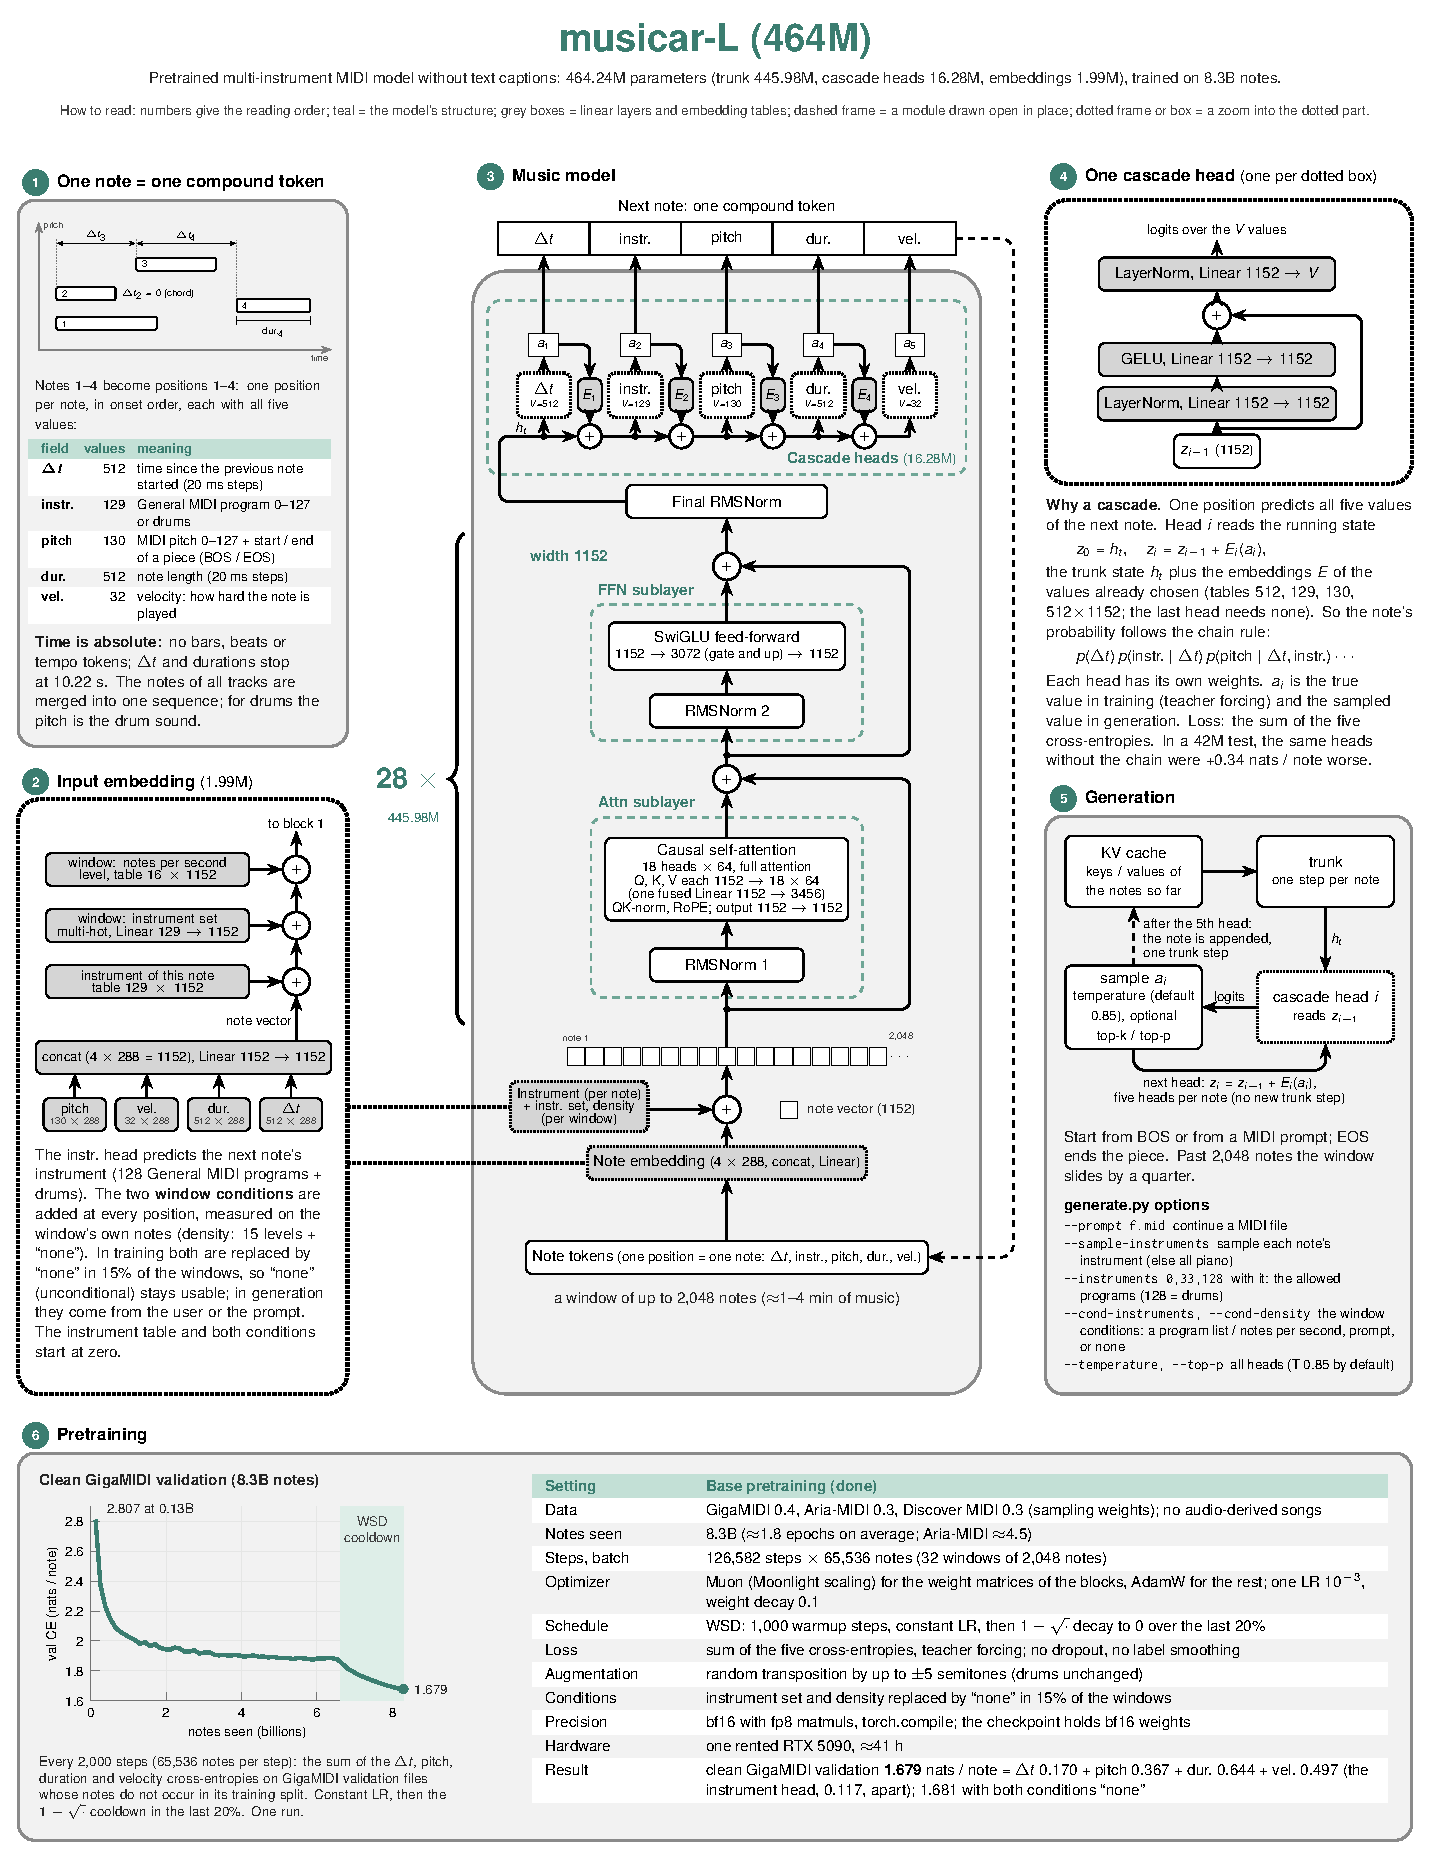
\includegraphics[scale=\dscale]{base_450m.pdf}}
\newsavebox{\bandBox}\sbox{\bandBox}{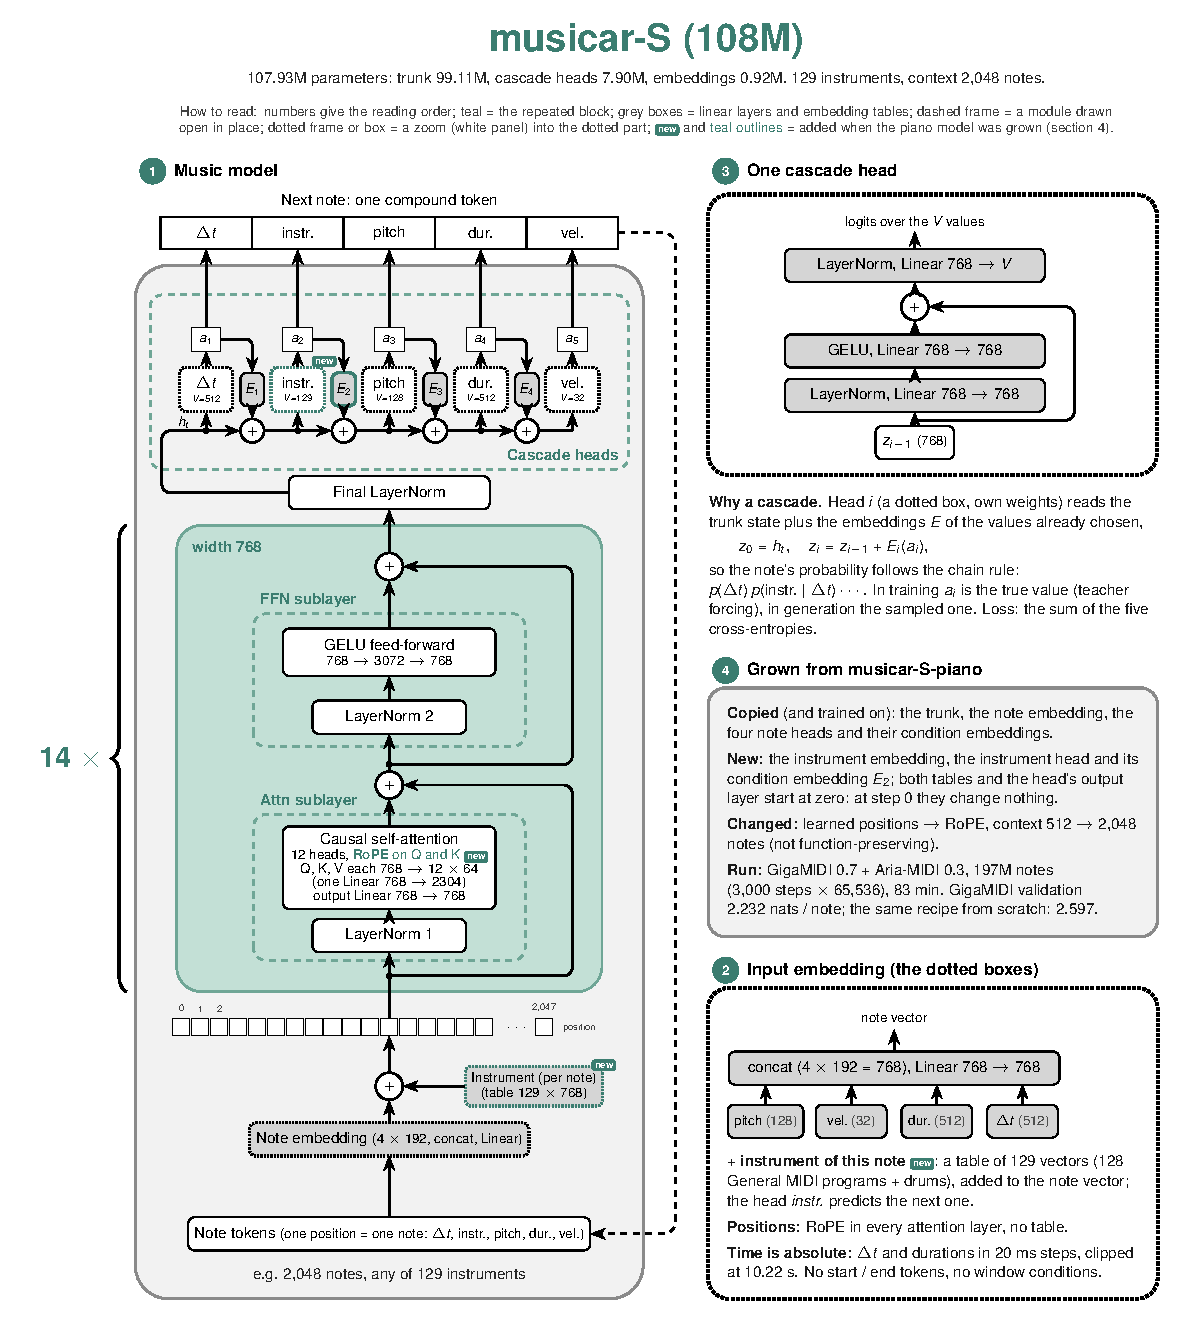
\includegraphics[scale=\dscale]{base_107m_band.pdf}}
\newsavebox{\pianoBox}\sbox{\pianoBox}{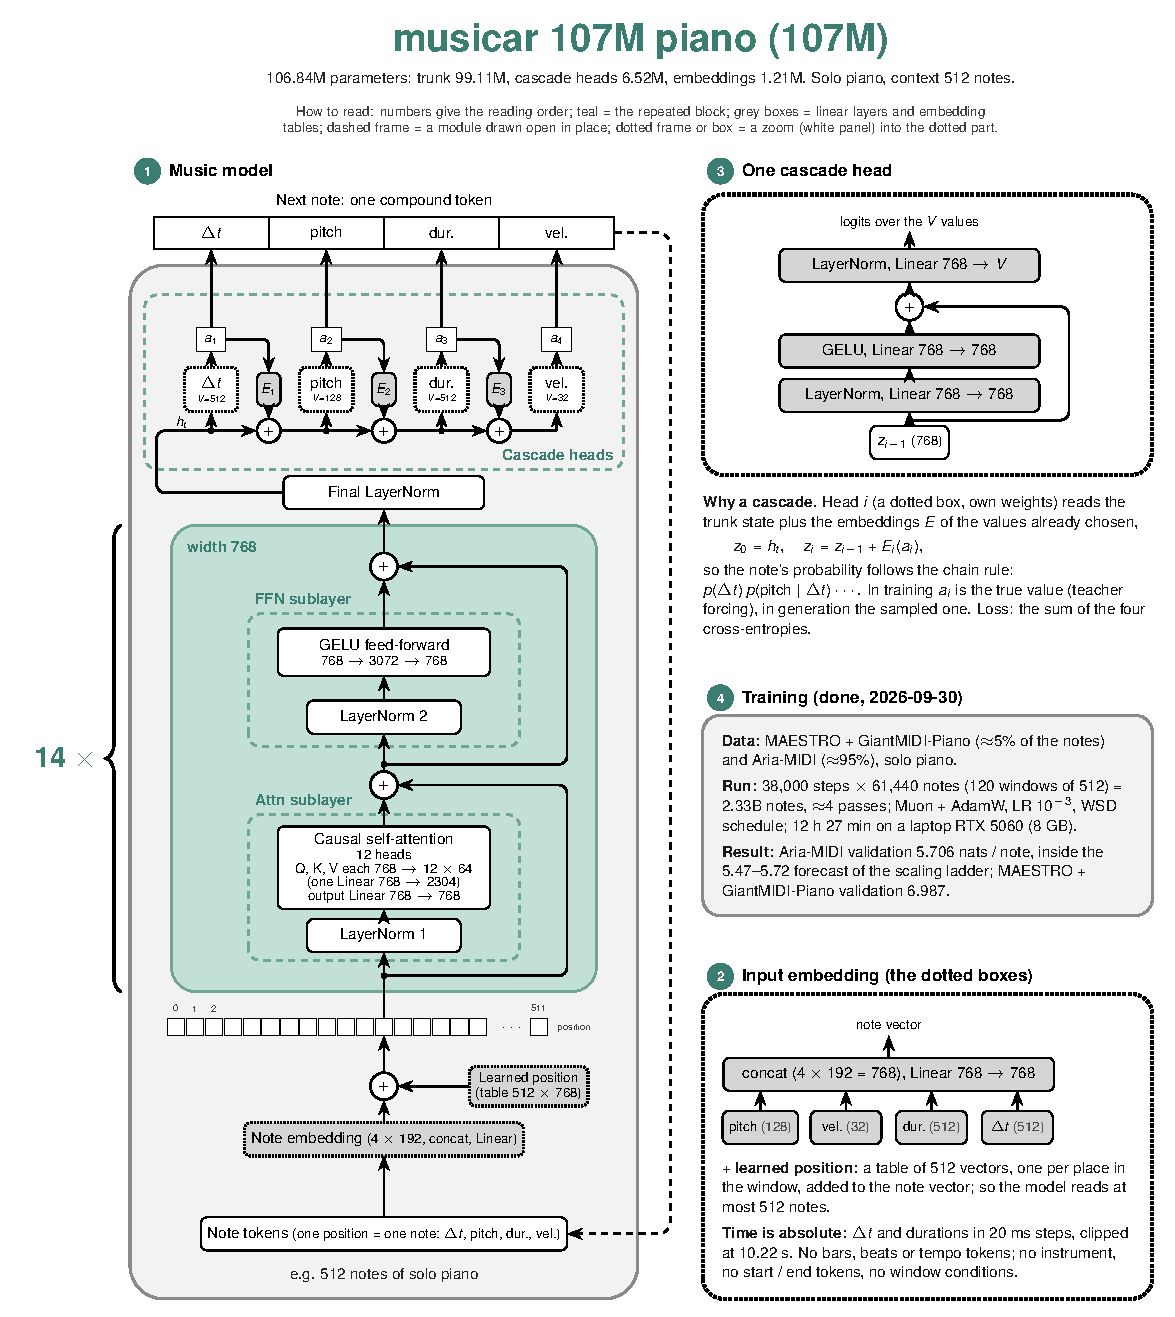
\includegraphics[scale=\dscale]{base_107m_piano.pdf}}
\newlength{\gapW}\setlength{\gapW}{0.9cm}
\newlength{\cmpW}\setlength{\cmpW}{\dimexpr\wd\bandBox + \gapW + \wd\pianoBox\relax}
\newlength{\boxesW}\setlength{\boxesW}{\dimexpr\wd\bigBox + \cmpW + \gapW - 3.3cm - 48pt\relax}

%% ================= comparison table (as wide as the two 107M diagrams) =================
\newsavebox{\cmpBox}
\sbox{\cmpBox}{\footnotesize\renewcommand{\arraystretch}{1.3}%
\begin{tabularx}{\cmpW}{@{\hspace{7pt}}>{\raggedright}p{2.05cm}>{\raggedright}X>{\raggedright}X>{\raggedright\arraybackslash}X@{\hspace{7pt}}}
\rowcolor{tealF} & \textcolor{tealT}{\textbf{musicar 450M base}} & \textcolor{tealT}{\textbf{musicar 107M band}} &
  \textcolor{tealT}{\textbf{musicar 107M piano}}\\
Parameters & 464.24M: trunk 445.98M, cascade heads 16.28M, embeddings 1.99M &
  107.93M: trunk 99.11M, cascade heads 7.90M, embeddings 0.92M &
  106.84M: trunk 99.11M, cascade heads 6.52M, embeddings 1.21M\\
\rowcolor{rowG}Trunk & 28 blocks, width 1152, 18 attention heads & 14 blocks, width 768, 12 attention heads &
  14 blocks, width 768, 12 attention heads\\
Context & 2,048 notes & 2,048 notes & 512 notes\\
\rowcolor{rowG}Instruments & 129 (128 General MIDI programs + drums), BOS / EOS, window conditions (instrument set, density) &
  129 (128 General MIDI programs + drums); no BOS / EOS, no conditions & piano only; no BOS / EOS, no conditions\\
Positions & RoPE & RoPE (replaced the piano model's learned table) & learned table ($512\times768$)\\
\rowcolor{rowG}Norm / MLP & RMSNorm, SwiGLU, QK-norm & LayerNorm, GELU & LayerNorm, GELU\\
Data & GigaMIDI 0.4, Aria-MIDI 0.3, Discover MIDI 0.3 & grown from the 107M piano, then GigaMIDI 0.7,
  Aria-MIDI 0.3 & MAESTRO + GiantMIDI-Piano $\approx$5\%, Aria-MIDI $\approx$95\%\\
\rowcolor{rowG}Notes seen & 8.3B (126,582 steps, $\approx$41 h on one RTX 5090) & 197M (3,000 steps, 83 min on a laptop RTX 5060),
  after the piano model's 2.33B & 2.33B (38,000 steps, 12 h 27 min on a laptop RTX 5060)\\
Result & clean GigaMIDI validation \textbf{1.679} & GigaMIDI validation \textbf{2.232} (older split that
  shares files with training) & Aria-MIDI validation \textbf{5.706} (512-note windows)\\
\end{tabularx}}

\begin{tikzpicture}

%% ================= title =================
\coordinate (O) at (0, 0);
\node[anchor=north west, inner sep=0pt] (big) at (O) {\usebox{\bigBox}};
\node[anchor=north west, inner sep=0pt] (band) at ([xshift=\gapW]big.north east) {\usebox{\bandBox}};
\node[anchor=north west, inner sep=0pt] (piano) at ([xshift=\gapW]band.north east) {\usebox{\pianoBox}};
\path (big.north west) -- (piano.north east) coordinate[pos=0.5] (Tmid);
\node[anchor=south, font=\fontsize{26}{30}\selectfont\bfseries, text=tealT] (title) at ([yshift=1.5cm]Tmid) {musicar pretrained bases};
\node[anchor=north, font=\small, text=black!85] at ([yshift=-0.15cm]title.south) {Three decoder-only transformers over
  compound note tokens (one position = one note, 20 ms grid), pretrained without captions. Each diagram has its own key.};

%% ================= comparison (under the two 107M diagrams) =================
\node[ptitle] (cmpT) at ([yshift=-1.0cm]band.south west) {Comparison};
\begin{scope}
  \clip[rounded corners=8pt] (cmpT.south west) rectangle ++(\wd\cmpBox, -\ht\cmpBox-\dp\cmpBox);
  \node[anchor=north west, inner sep=0pt] (cmp) at (cmpT.south west) {\usebox{\cmpBox}};
\end{scope}
\draw[rounded corners=8pt, draw=greyB, line width=1pt] (cmp.south west) rectangle (cmp.north east);
\node[anchor=north west, text width=\wd\cmpBox, font=\scriptsize, text=black!80, align=flush left, inner sep=0pt]
  (cmpN) at ([yshift=-0.2cm]cmp.south west) {Result: validation cross-entropy in nats per note (teacher-forced, summed
  over $\Delta t$, pitch, duration and velocity; lower is better). The three validation sets differ, so the numbers are
  not comparable across columns.};

%% ================= next steps (planned) =================
\path let \p1 = (big.south), \p2 = (cmpN.south) in coordinate (N) at (0, {min(\y1, \y2) - 1.0cm});
\node[ptitle] (nextT) at (N) {Next (planned, not done)};
\begin{scope}[node distance=1.1cm]
  \node[box, anchor=north west, text width=0.15\boxesW, minimum height=13mm] (n0) at ([yshift=-0.25cm]nextT.south west)
    {\textbf{musicar 450M base} (done)\\[-1pt] {\scriptsize pretrained, no captions}};
  \node[box, right=of n0, text width=0.31\boxesW, minimum height=13mm] (n1)
    {\textbf{F1: the captioned 450M}\\[-1pt] {\scriptsize captions from a frozen multilingual LaBSE encoder (English and
    Ukrainian), section captions, length control; the recipe is being settled in laptop pilots}};
  \node[box, right=of n1, text width=0.24\boxesW, minimum height=13mm] (n2)
    {\textbf{F2: the Ukrainian captioned fine-tune}\\[-1pt] {\scriptsize F1 fine-tuned on about 5,400 Ukrainian songs
    transcribed from audio}};
  \node[box, dashed, draw=black!60, right=of n2, text width=0.30\boxesW, minimum height=13mm, text=black!85] (n3)
    {\textbf{The 107M bases are not trained further}\\[-1pt] {\scriptsize they stay as small, cheap bases for pilots:
    the 107M band carries the caption pilots that settle F1's recipe}};
  \draw[arr] (n0) -- (n1);
  \draw[arr] (n1) -- (n2);
  \draw[arr, dashed, black!60, rounded corners=5pt] (n3.north) -- ++(0, 0.45) -| node[pos=0.25, above, font=\scriptsize,
    text=black!75] {pilots} (n1.north);
\end{scope}

\end{tikzpicture}
\end{document}
